\section{Tournament Analysis}

\subsection{Our expectation}
One principle of our approach is, make no assumption on the distribution.
All strategies that we use aim to maximize the freedom of future building placement.
So we expect that our player would perform consistently well against every possible adversarial distribution.

Because we didn't do any optimization to some specific distributions. It's performance may not be so good if
the underline distribution has some simple ``optimal solution". But we tends to let the problem itself to decide
which placement is ``better", instead of giving too specific instructions in some situations.

\subsection{Performance}

The result of the tournament is close to what we have expected.
Despite the fact that our player's performance is quite well: it has the second best winning rounds (34, the
first wins 37 rounds), and also the second best average score (1980.55, we'll explain why it's not the highest later).
We want to highlight the one property of our player, that is ``robustness".

\begin{figure}[ht]
\centering
\begin{subfigure}[t]{.45\textwidth}
\centering
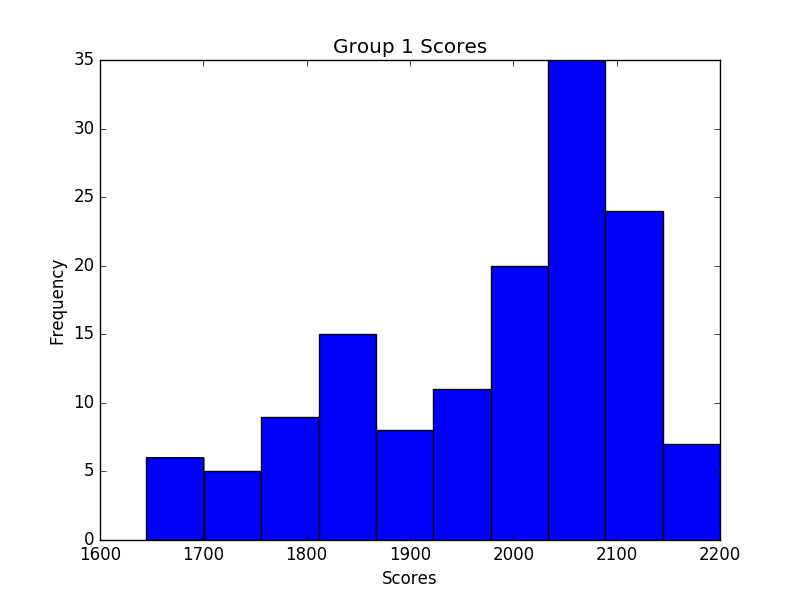
\includegraphics[width=\textwidth]{Histograms/g1.png}
\end{subfigure}
~
\begin{subfigure}[t]{.45\textwidth}
\centering
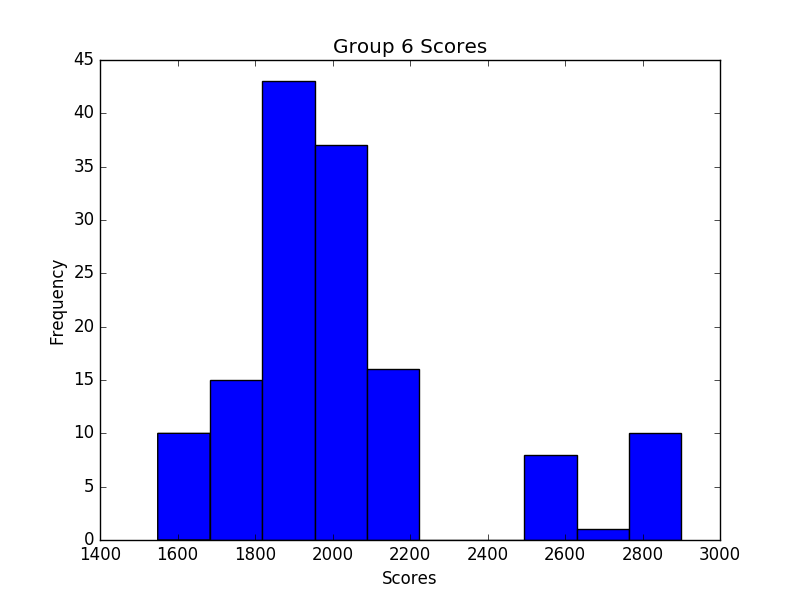
\includegraphics[width=\textwidth]{Histograms/g6.png}
\end{subfigure}
\caption{Score distribution of player 1 (left) and the highest average score player (right)}\label{fig:scores}
\end{figure}

First figure~\ref{fig:scores} shows the score distribution of our player. Most of our scores are concenterated above
2000. Which makes our player has the highest median score as in figure~\ref{fig:median}. 
One interesting fact about the highest average score player is, its score distribution has some isolated
``very high" part, where we believe is the key of getting the highest average score.

Figure~\ref{fig:average} shows that, on almost every distribution, our performance is significantly higher than
the average. It demonstrates the benefits if your strategy is robust and does not depend on the distribution.
A more detailed table is listed in figure~\ref{fig:table}. If we average the scores for each distribution, our
player wins 4 distributions and it's a tie with group 6. (While if you look into the distribution presented by
group 6 and group 9, you'll find out that they are exactly the target distributions for group 6's strategy).

We also perform an 1-vs-1 match analysis over the tournament result. It's more like the rules of modern football leagues,
we perform a round robin for all the players and see the comparison between every pairs of them.
The result is shown in table~\ref{fig:scoretable}. Clearly that our player, which we believe is the most robust one,
wins every match of the tournament.

\begin{figure}[t]
\begin{center}
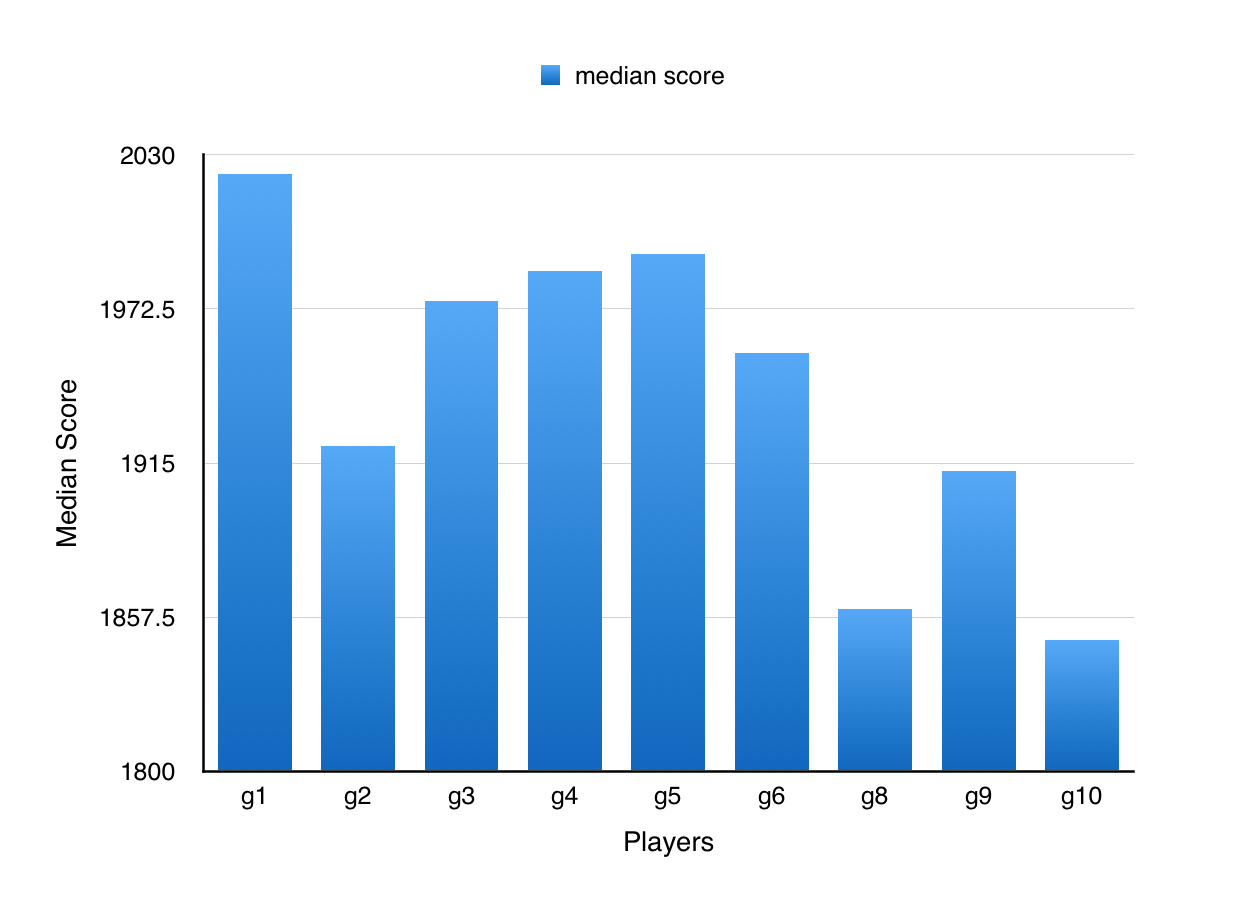
\includegraphics[width=0.48\linewidth]{median.png}
\end{center}
\caption{Median scores of each player}\label{fig:median}
\end{figure}


\begin{figure}[ht]
\begin{center}
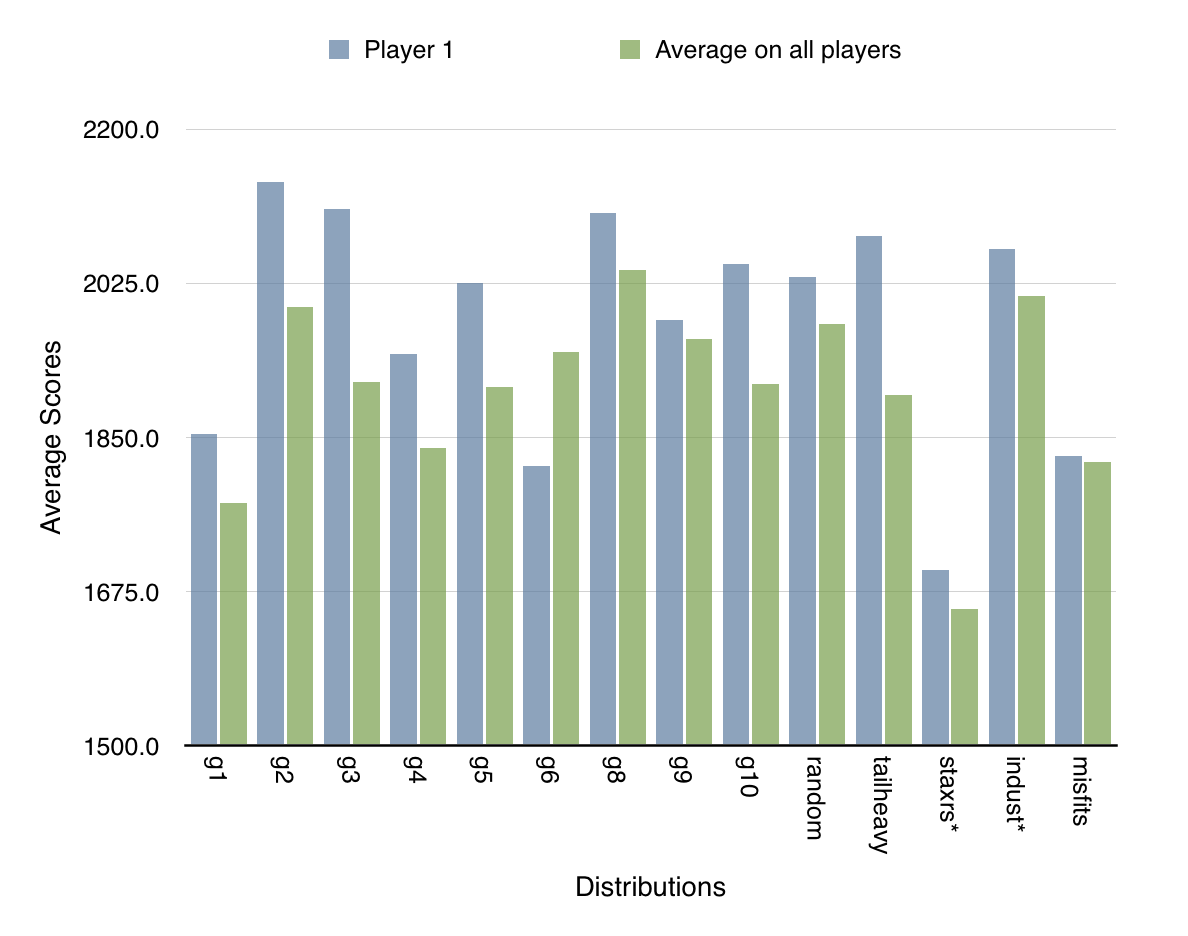
\includegraphics[width=0.48\linewidth]{average.png}
\end{center}
\caption{Averge scores of player 1 on each distribution}\label{fig:average}
\end{figure}

\begin{table}[ht]
\centering
%\begin{tabular}{| l | @{}c | @{}c | @{}c | @{}c | @{}c | @{}c | @{}c | @{}c | @{}c | @{}c |}
%\hline
%Sequencer & g1 & g2 & g3 & g4 & g5 & g6 & g8 & g9 & g10 & average \\
%\hline
%g1 & 1853.6 & 1784.1 & 1776.5 & 1823.4 & {\bf \color{red} 1865.8} & 1796 & 1692.5 & 1762.7 & 1621.8 & 1775.2 \\
%\hline
%g2 & {\bf \color{red} 2140.2} & 2005 & 2055.2 & 2043.2 & 1942 & 1948.2 & 1999.8 & 2022 & 1830 & 1998.4 \\
%\hline
%g3 & {\bf \color{red} 2109.2} & 1947.7 & 1410.5 & 2006.2 & 2094.4 & 1941.8 & 1722 & 2023.7 & 1961.9 & 1913.0 \\
%\hline
%g4 & {\bf \color{red} 1944.3} & 1872.7 & 1714.7 & 1890 & 1940.9 & 1826.6 & 1781.4 & 1823.4 & 1748.7 & 1838.1 \\
%\hline
%g5 & 2025.6 & 1900.3 & 1661.2 & 1963.2 & {\bf \color{red} 2120.2} & 1905.6 & 1755.2 & 1957.2 & 1872.8 & 1906.8 \\
%\hline
%g6 & 1817.6 & 1893.4 & 1494.1 & 2004.4 & 1943 & {\bf \color{red} 2900} & 1830.7 & 1788 & 1849 & 1946.7 \\
%\hline
%g8 & 2104.5 & 2030.6 & 2065.1 & 2018.5 & 2033.4 & 2046.3 & {\bf \color{red} 2140.9} & 2022.9 & 1894.5 & 2039.6 \\
%\hline
%g9 & 1983.6 & 1917.3 & 1713.1 & 1987.1 & 1952.3 & {\bf \color{red} 2532.3} & 1962.5 & 1809.6 & 1801.6 & 1962.2 \\
%\hline
%g10& {\bf \color{red} 2046.9} & 1905.7 & 1729.1 & 1923.7 & 2042.8 & 1863 & 1885.2 & 1889.4 & 1912 & 1910.9 \\
%\hline
%random &2031.7 & 1983 & 2067.2 & 2046.3 & 2020.1 & {\bf \color{red} 2069.9} & 1615.3 & 2029.8 & 1939.7 & 1978.1 \\
%\hline
%tailheavy &2078.5 & 2010.1 & {\bf \color{red} 2119.9} & 2083.9 & 2067 & 2097.3 & 615.7 & 2057.8 & 1950.3 & 1897.8 \\
%\hline
%stars* &1699 & 1672.4 & 1681.2 & 1697 & {\bf \color{red} 1807.2} & 1584.1 & 1656.1 & 1588.1 & 1513.2 & 1655.4 \\
%\hline
%indust* &2064.4 & 2001 & 2089.4 & 2029 & 2054 & {\bf \color{red} 2093.2} & 1811.6 & 2032.1 & 1915.4 & 2010.0 \\
%\hline
%misfits &1828.6 & 1822.8 & 1830.1 & {\bf \color{red} 1899.8} & 1778.9 & 1881.8 & 1816.2 & 1839.9 & 1703.1 & 1822.4 \\
%\hline
%\end{tabular}
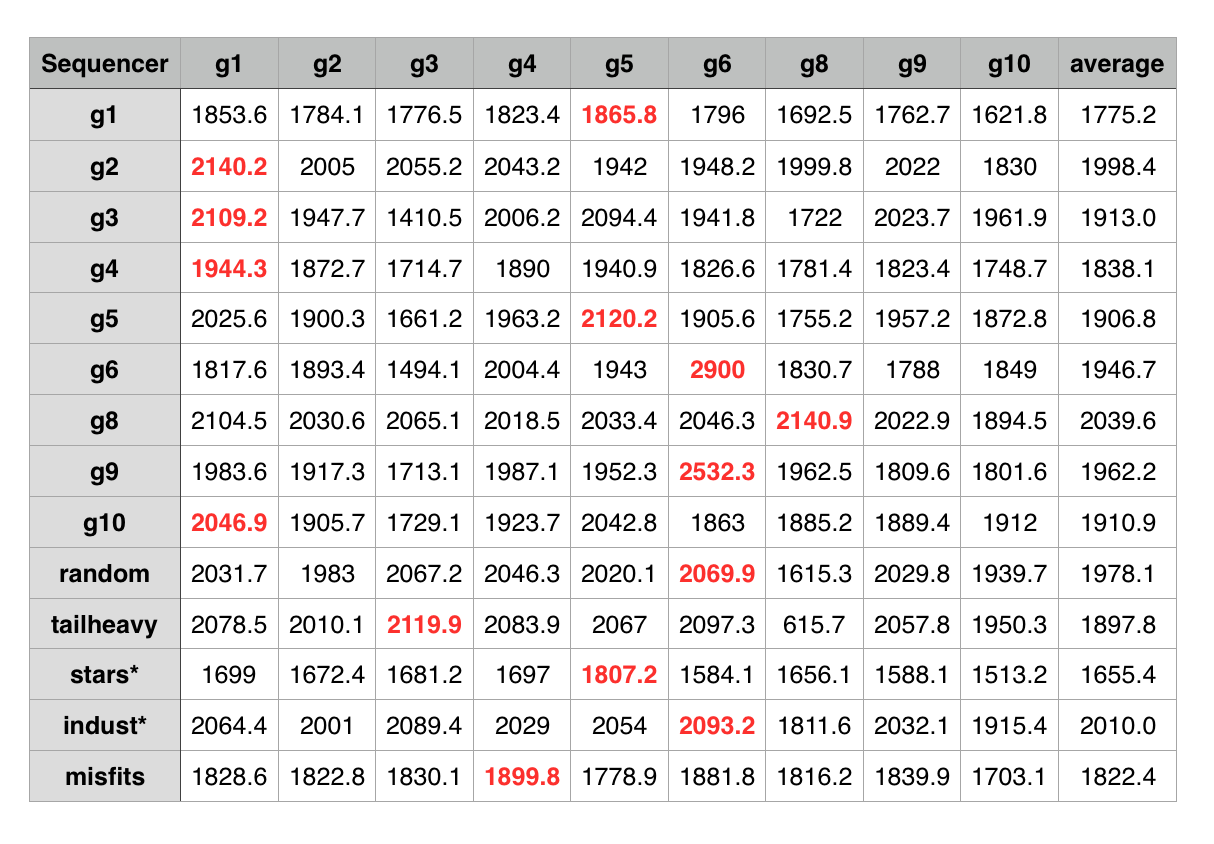
\includegraphics[width=0.9\linewidth]{avgtable.png}
\caption{Average scores of each player running on each distribution. \newline
The {\bf \color{red} bold red} ones are the distribution winner.}\label{fig:table}
\end{table}

\begin{table}[ht]
\centering
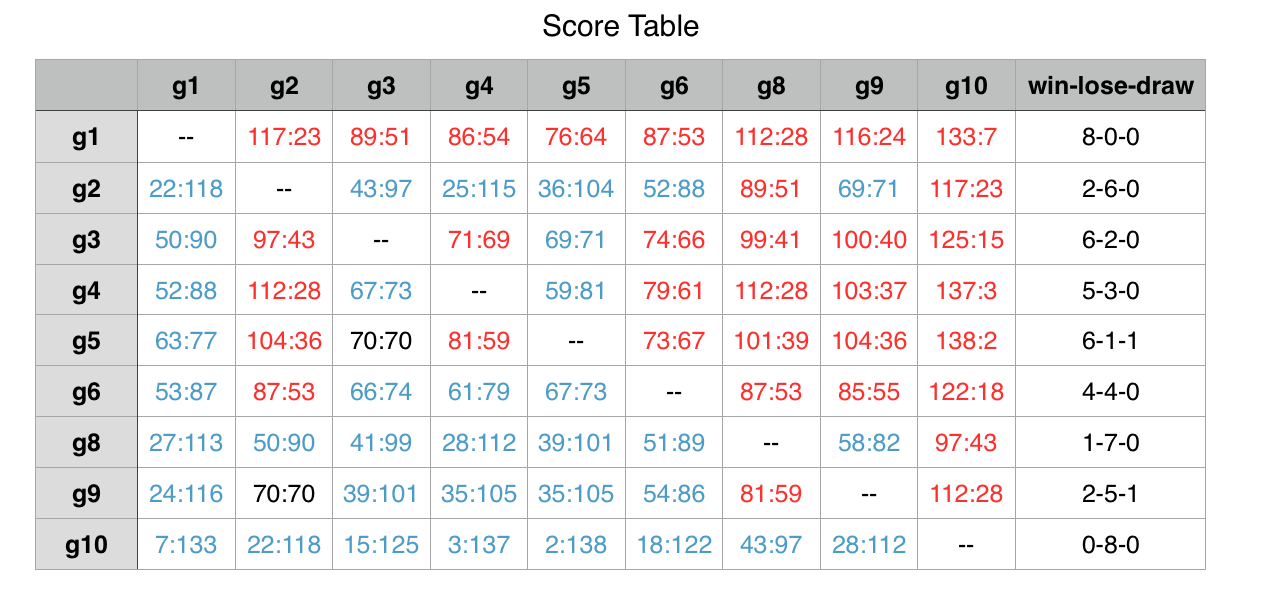
\includegraphics[width=0.9\linewidth]{scoretablerevise.png}
\caption{Score table of pairwise comparison}\label{fig:scoretable}
\end{table}

